
\documentclass[letterpaper,hide notes,xcolor={table,svgnames},pdftex,10pt]{beamer}
\def\showexamples{t}


%\usepackage[svgnames]{xcolor}

%% Demo talk
%\documentclass[letterpaper,notes=show]{beamer}

\usecolortheme{crane}
\setbeamertemplate{navigation symbols}{}

\usetheme{MyPittsburgh}
%\usetheme{Frankfurt}

%\usepackage{tipa}

\usepackage{hyperref}
\usepackage{graphicx,xspace}
\usepackage[normalem]{ulem}

\newcommand\SF[1]{$\bigstar$\footnote{SF: #1}}

\usepackage[default]{sourcesanspro}
\usepackage[T1]{fontenc}

\newcounter{tmpnumSlide}
\newcounter{tmpnumNote}

% old question code
%\newcommand\question[1]{{$\bigstar$ \small \onlySlide{2}{#1}}}
% \newcommand\nquestion[1]{\ifdefined \presentationonly \textcircled{?} \fi \note{\par{\Large \textbf{?}} #1}}
% \newcommand\nanswer[1]{\note{\par{\Large \textbf{A}} #1}}


 \newcommand\mnote[1]{%
   \addtocounter{tmpnumSlide}{1}
   \ifdefined\showcues {~\tiny\fbox{\arabic{tmpnumSlide}}}\fi
   \note{\setlength{\parskip}{1ex}\addtocounter{tmpnumNote}{1}\textbf{\Large \arabic{tmpnumNote}:} {#1\par}}}

\newcommand\mmnote[1]{\note{\setlength{\parskip}{1ex}#1\par}}

%\newcommand\mnote[2][]{\ifdefined\handoutwithnotes {~\tiny\fbox{#1}}\fi
% \note{\setlength{\parskip}{1ex}\textbf{\Large #1:} #2\par}}

%\newcommand\mnote[2][]{{\tiny\fbox{#1}} \note{\setlength{\parskip}{1ex}\textbf{\Large #1:} #2\par}}

\newcommand\mquestion[2]{{~\color{red}\fbox{?}}\note{\setlength{\parskip}{1ex}\par{\Large \textbf{?}} #1} \note{\setlength{\parskip}{1ex}\par{\Large \textbf{A}} #2\par}\ifdefined \presentationonly \pause \fi}

\newcommand\blackboard[1]{%
\ifdefined   \showblackboard
  {#1}
  \else {\begin{center} \fbox{\colorbox{blue!30}{%
         \begin{minipage}{.95\linewidth}%
           \hspace{\stretch{1}} Some space intentionally left blank; done at the blackboard.%
         \end{minipage}}}\end{center}}%
         \fi%
}



%\newcommand\q{\tikz \node[thick,color=black,shape=circle]{?};}
%\newcommand\q{\ifdefined \presentationonly \textcircled{?} \fi}

\usepackage{listings}
\lstset{%
  keywordstyle=\bfseries,
  aboveskip=15pt,
  belowskip=15pt,
  captionpos=b,
  identifierstyle=\ttfamily,
  escapeinside={(*@}{@*)},
  stringstyle=\ttfamiliy,
  frame=lines,
  numbers=left, basicstyle=\scriptsize, numberstyle=\tiny, stepnumber=0, numbersep=2pt}

\usepackage{siunitx}
\newcommand\sius[1]{\num[group-separator = {,}]{#1}\si{\micro\second}}
\newcommand\sims[1]{\num[group-separator = {,}]{#1}\si{\milli\second}}
\newcommand\sins[1]{\num[group-separator = {,}]{#1}\si{\nano\second}}
\sisetup{group-separator = {,}, group-digits = true}

%% -------------------- tikz --------------------
\usepackage{tikz}
\usetikzlibrary{positioning}
\usetikzlibrary{arrows,backgrounds,automata,decorations.shapes,decorations.pathmorphing,decorations.markings,decorations.text}

\tikzstyle{place}=[circle,draw=blue!50,fill=blue!20,thick, inner sep=0pt,minimum size=6mm]
\tikzstyle{transition}=[rectangle,draw=black!50,fill=black!20,thick, inner sep=0pt,minimum size=4mm]

\tikzstyle{block}=[rectangle,draw=black, thick, inner sep=5pt]
\tikzstyle{bullet}=[circle,draw=black, fill=black, thin, inner sep=2pt]

\tikzstyle{pre}=[<-,shorten <=1pt,>=stealth',semithick]
\tikzstyle{post}=[->,shorten >=1pt,>=stealth',semithick]
\tikzstyle{bi}=[<->,shorten >=1pt,shorten <=1pt, >=stealth',semithick]

\tikzstyle{mut}=[-,>=stealth',semithick]

\tikzstyle{treereset}=[dashed,->, shorten >=1pt,>=stealth',thin]

\usepackage{ifmtarg}
\usepackage{xifthen}
\makeatletter
% new counter to now which frame it is within the sequence
\newcounter{multiframecounter}
% initialize buffer for previously used frame title
\gdef\lastframetitle{\textit{undefined}}
% new environment for a multi-frame
\newenvironment{multiframe}[1][]{%
\ifthenelse{\isempty{#1}}{%
% if no frame title was set via optional parameter,
% only increase sequence counter by 1
\addtocounter{multiframecounter}{1}%
}{%
% new frame title has been provided, thus
% reset sequence counter to 1 and buffer frame title for later use
\setcounter{multiframecounter}{1}%
\gdef\lastframetitle{#1}%
}%
% start conventional frame environment and
% automatically set frame title followed by sequence counter
\begin{frame}%
\frametitle{\lastframetitle~{\normalfont(\arabic{multiframecounter})}}%
}{%
\end{frame}%
}
\makeatother

\makeatletter
\newdimen\tu@tmpa%
\newdimen\ydiffl%
\newdimen\xdiffl%
\newcommand\ydiff[2]{%
    \coordinate (tmpnamea) at (#1);%
    \coordinate (tmpnameb) at (#2);%
    \pgfextracty{\tu@tmpa}{\pgfpointanchor{tmpnamea}{center}}%
    \pgfextracty{\ydiffl}{\pgfpointanchor{tmpnameb}{center}}%
    \advance\ydiffl by -\tu@tmpa%
}
\newcommand\xdiff[2]{%
    \coordinate (tmpnamea) at (#1);%
    \coordinate (tmpnameb) at (#2);%
    \pgfextractx{\tu@tmpa}{\pgfpointanchor{tmpnamea}{center}}%
    \pgfextractx{\xdiffl}{\pgfpointanchor{tmpnameb}{center}}%
    \advance\xdiffl by -\tu@tmpa%
}
\makeatother
\newcommand{\copyrightbox}[3][r]{%
\begin{tikzpicture}%
\node[inner sep=0pt,minimum size=2em](ciimage){#2};
\usefont{OT1}{phv}{n}{n}\fontsize{4}{4}\selectfont
\ydiff{ciimage.south}{ciimage.north}
\xdiff{ciimage.west}{ciimage.east}
\ifthenelse{\equal{#1}{r}}{%
\node[inner sep=0pt,right=1ex of ciimage.south east,anchor=north west,rotate=90]%
{\raggedleft\color{black!50}\parbox{\the\ydiffl}{\raggedright{}#3}};%
}{%
\ifthenelse{\equal{#1}{l}}{%
\node[inner sep=0pt,right=1ex of ciimage.south west,anchor=south west,rotate=90]%
{\raggedleft\color{black!50}\parbox{\the\ydiffl}{\raggedright{}#3}};%
}{%
\node[inner sep=0pt,below=1ex of ciimage.south west,anchor=north west]%
{\raggedleft\color{black!50}\parbox{\the\xdiffl}{\raggedright{}#3}};%
}
}
\end{tikzpicture}
}


%% --------------------

%\usepackage[excludeor]{everyhook}
%\PushPreHook{par}{\setbox0=\lastbox\llap{MUH}}\box0}

%\vspace*{\stretch{1}

%\setbox0=\lastbox \llap{\textbullet\enskip}\box0}

\setlength{\parskip}{\fill}

\newcommand\noskips{\setlength{\parskip}{1ex}}
\newcommand\doskips{\setlength{\parskip}{\fill}}

\newcommand\xx{\par\vspace*{\stretch{1}}\par}
\newcommand\xxs{\par\vspace*{2ex}\par}
\newcommand\tuple[1]{\langle #1 \rangle}
\newcommand\code[1]{{\sf \footnotesize #1}}
\newcommand\ex[1]{\uline{Example:} \ifdefined \presentationonly \pause \fi
  \ifdefined\showexamples#1\xspace\else{\uline{\hspace*{2cm}}}\fi}

\newcommand\ceil[1]{\lceil #1 \rceil}


\AtBeginSection[]
{
   \begin{frame}
       \frametitle{Outline}
       \tableofcontents[currentsection]
   \end{frame}
}



\pgfdeclarelayer{edgelayer}
\pgfdeclarelayer{nodelayer}
\pgfsetlayers{edgelayer,nodelayer,main}

\tikzstyle{none}=[inner sep=0pt]
\tikzstyle{rn}=[circle,fill=Red,draw=Black,line width=0.8 pt]
\tikzstyle{gn}=[circle,fill=Lime,draw=Black,line width=0.8 pt]
\tikzstyle{yn}=[circle,fill=Yellow,draw=Black,line width=0.8 pt]
\tikzstyle{empty}=[circle,fill=White,draw=Black]
\tikzstyle{bw} = [rectangle, draw, fill=blue!20, 
    text width=4em, text centered, rounded corners, minimum height=2em]
    
    \newcommand{\CcNote}[1]{% longname
	This work is licensed under the \textit{Creative Commons #1 3.0 License}.%
}
\newcommand{\CcImageBy}[1]{%
	\includegraphics[scale=#1]{creative_commons/cc_by_30.pdf}%
}
\newcommand{\CcImageSa}[1]{%
	\includegraphics[scale=#1]{creative_commons/cc_sa_30.pdf}%
}
\newcommand{\CcImageNc}[1]{%
	\includegraphics[scale=#1]{creative_commons/cc_nc_30.pdf}%
}
\newcommand{\CcGroupBySa}[2]{% zoom, gap
	\CcImageBy{#1}\hspace*{#2}\CcImageNc{#1}\hspace*{#2}\CcImageSa{#1}%
}
\newcommand{\CcLongnameByNcSa}{Attribution-NonCommercial-ShareAlike}

\newenvironment{changemargin}[1]{% 
  \begin{list}{}{% 
    \setlength{\topsep}{0pt}% 
    \setlength{\leftmargin}{#1}% 
    \setlength{\rightmargin}{1em}
    \setlength{\listparindent}{\parindent}% 
    \setlength{\itemindent}{\parindent}% 
    \setlength{\parsep}{\parskip}% 
  }% 
  \item[]}{\end{list}} 




\title{Lecture 8 --- Threads}

\author{Jeff Zarnett \\ \small \texttt{jzarnett@uwaterloo.ca}}
\institute{Department of Electrical and Computer Engineering \\
  University of Waterloo}
\date{\today}


\begin{document}

\begin{frame}
  \titlepage

 \end{frame}

\begin{frame}
\frametitle{What is a Thread?}


Recall our earlier examination of the process. 

A process has three major components: 
\begin{enumerate}
\item An executable program;
\item The data created/needed by the program; and 
\item The execution context of the program.
\end{enumerate}

A process has at least one \alert{thread}, and can have many.

\end{frame}

\begin{frame}
\frametitle{What is a Thread?}

The term ``thread'' is a short form of \alert{Thread of Execution}.

  A thread of execution is a sequence of executable commands that can be scheduled to run on the CPU. 
  
  Threads also have some state and stores some local variables.
  
  Most programs you will write in other courses had only one thread;\\
  \quad that is, your program's code is executed one statement at a time.

\end{frame}

\begin{frame}
\frametitle{Multithreaded Programs}

A multithreaded program uses more than one thread, (some of the time).

  A program begins with an initial thread (where the \texttt{main} method is).
  
That main thread can create some additional threads if needed.

 Threads can be created and destroyed within a program dynamically.

\end{frame}

\begin{frame}
\frametitle{Threads and Processes}

\begin{center}
	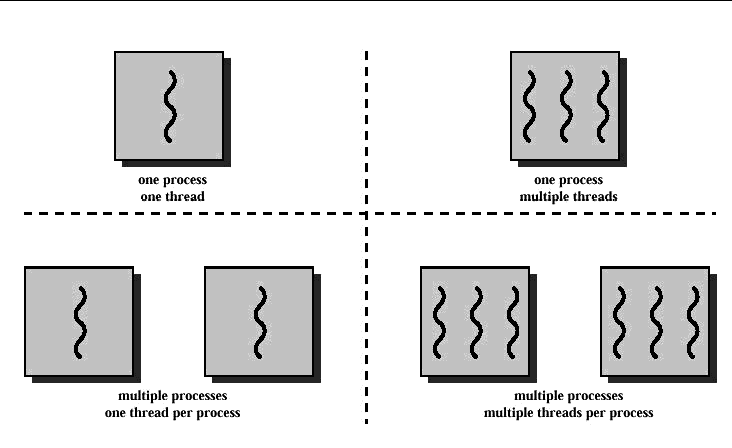
\includegraphics[width=0.9\textwidth]{images/mthread.png}
\end{center}

\end{frame}

\begin{frame}
\frametitle{Thread Possessions}


In a process that has multiple threads, each thread has its own:
\begin{enumerate}
	\item Thread execution state.
	\item Saved thread context when not running.
	\item Execution stack.
	\item Local variables.
	\item Access to the memory and resources of the process (shared with all threads in that process).
\end{enumerate}

\end{frame}

\begin{frame}
\frametitle{Single vs. Multithreaded}

\begin{center}
	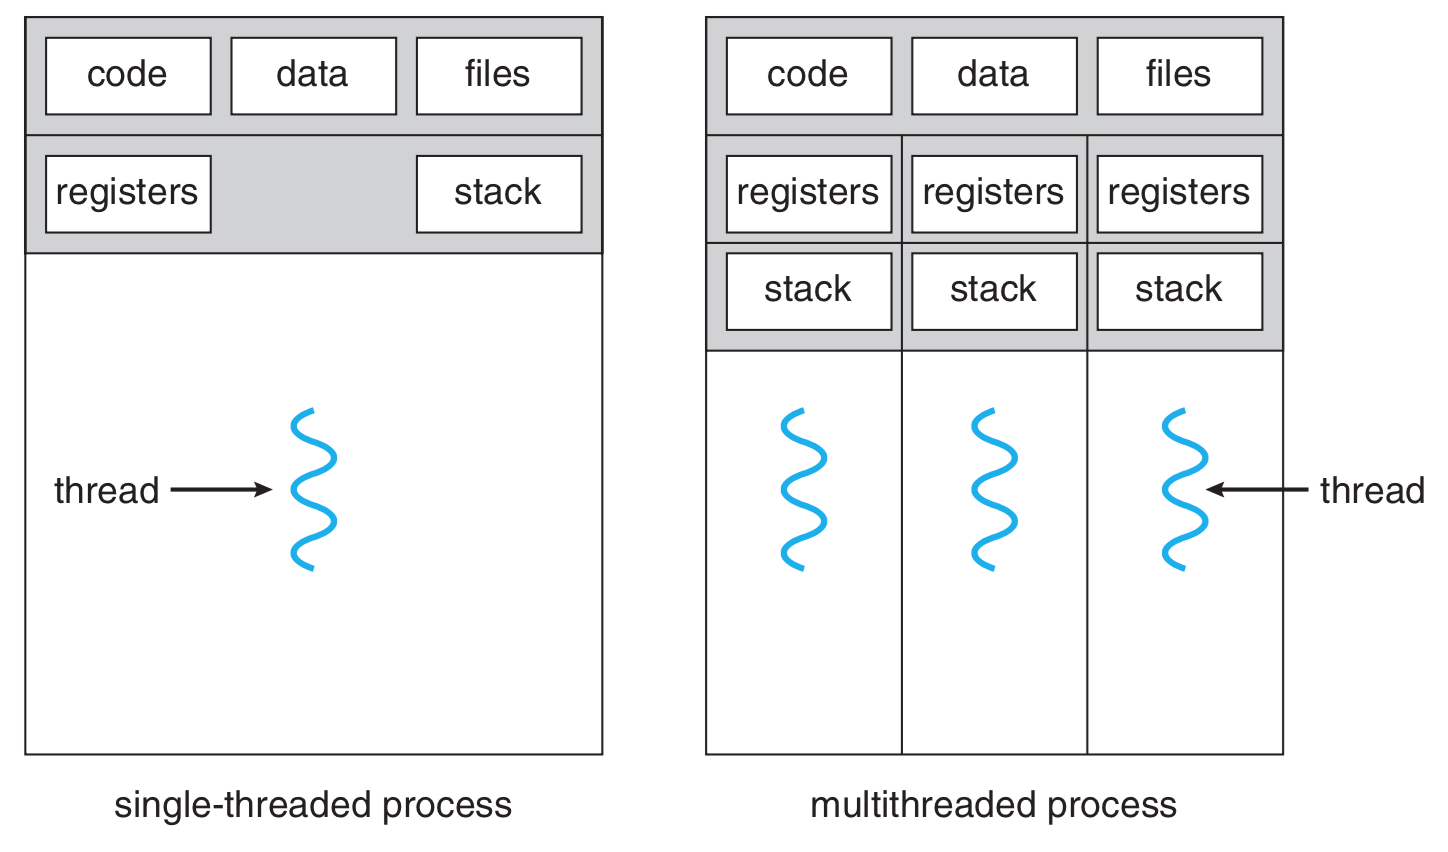
\includegraphics[width=0.9\textwidth]{images/mthread2.png}
\end{center}

\end{frame}

\begin{frame}
\frametitle{Thread Notes}

All the threads of a process share the state and resources of the process. 

If a thread opens a file, other threads in that process can also access it.

The way programs are written now, few are not multithreaded.



\end{frame}

\begin{frame}
\frametitle{UI Thread}

One common way of dividing up the program into threads is to separate the user interface from a time-consuming action. 

Consider a file-transfer program. 

If the user interface and upload method share a thread, once a file upload has started, the user will not be able to use the UI anymore.

Not even to click the button that cancels the upload! 

For some reason, users hate that. 

\end{frame}

\begin{frame}
\frametitle{Solving the UI Thread Problem}

We have two options for how to alleviate this problem.

Option 1: \texttt{fork} a new process to do the upload; or \\
Option 2: Spawn  new thread. 

In either case, the newly created entity will handle the upload of the file. 

The UI remains responsive, because the UI thread is not waiting for the upload method to complete.

\end{frame}

\begin{frame}
\frametitle{Thread Motivation}
Why threads instead of a new process?

Primary motivation is: performance.

\begin{enumerate}
	\item Creation: 10$\times$ faster.
	\item Terminating and cleaning up a thread is faster.
	\item Switch time: 20\% of process switch time.
	\item Shared memory space (no need for IPC).
	\item Lets the UI be responsive.
\end{enumerate}

\end{frame}

\begin{frame}
\frametitle{Common Usage of Threads}

\begin{enumerate}
	\item \textbf{Foreground and Background Work}
	\item \textbf{Asynchronous processing}
	\item \textbf{Speed of Execution}
	\item \textbf{Modular Structure}
\end{enumerate}

\end{frame}

\begin{frame}
\frametitle{Thread Drawbacks}

There is no protection between threads in the same process. 

One thread can easily mess with the memory being used by another. 

This once again brings us to the subject of co-ordination, which will follow the discussion of threads.

Also, if any thread encounters an error, the whole process might be terminated by the operating system.

\end{frame}

\begin{frame}
\frametitle{Thread States}
Each individual thread will have its own state. 

Our process model has seven states.\\
\quad The thread state model is the simpler five-state model. 

If a process is swapped out of memory, all its threads are swapped out.

When that process returns to memory, all the threads are swapped in.

Therefore we do not need to consider if a thread is in memory/swapped.

\end{frame}

\begin{frame}
\frametitle{Five State Model}
Five state model, once again:

\begin{center}
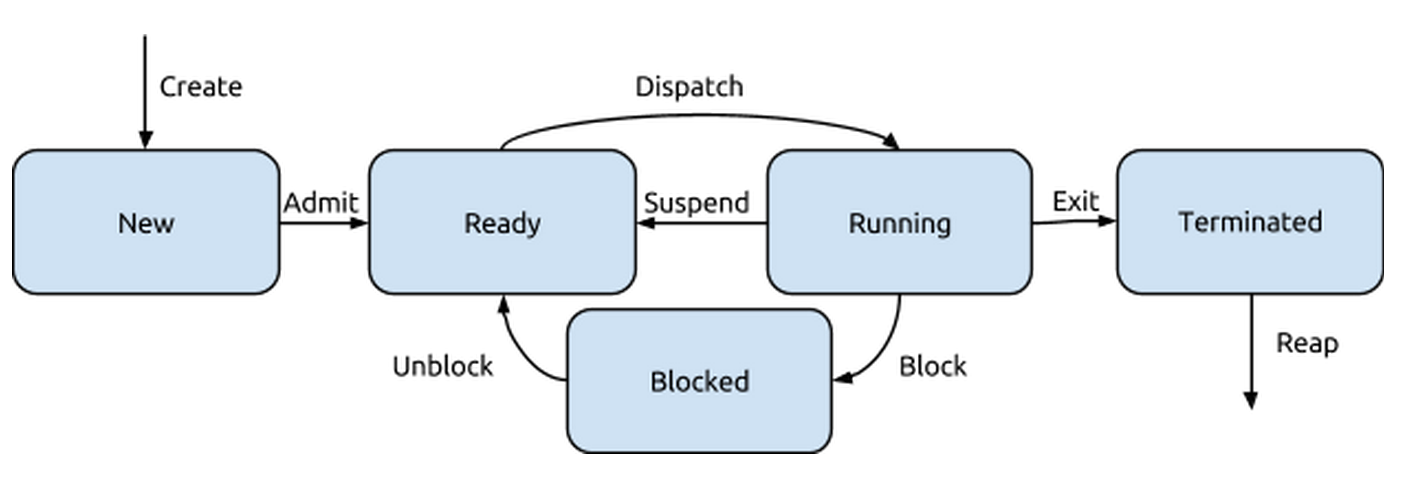
\includegraphics[width=0.85\textwidth]{images/5-state-model.png}
\end{center}

\end{frame}

\begin{frame}
\frametitle{Five State Model}

The transitions work the same way as the state transitions for a process. 

As with a process, a thread in any state can transition to terminated. W

hen a process is terminated, all its threads are terminated\\
\quad Regardless of what state it is in.

Actually, let's take a minute to look at cancellation...

\end{frame}

\begin{frame}
\frametitle{Thread Cancellation}

Thread cancellation is exactly what it sounds like. 

A running thread will be terminated before it has finished its work. 

Once the user presses the cancel button on the file upload, we want to stop the upload task that was in progress. 

The thread that we are going to cancel is called the \alert{target}.

\end{frame}

\begin{frame}
\frametitle{Thread Cancellation}

\begin{enumerate}
	\item \textbf{Asynchronous Cancellation}
	\item \textbf{Deferred Cancellation} 
\end{enumerate}

\end{frame}

\begin{frame}
\frametitle{Deferred Cancellation}

For example, in Android, a background task has a function \texttt{isCancelled}.

This function returns a boolean value. 

If we cancel a task then the \texttt{isCancelled} value returns true.\\
\quad That  on its own has no impact on the task. 

The task itself is responsible for checking if \texttt{isCancelled} is true.

Yes, a thread can just ignore the cancellation.

\end{frame}

\begin{frame}
\frametitle{Deferred Cancellation}

If a thread can ignore cancellation, why would we ever choose deferred? 

Suppose the thread we are cancelling has some resources. 

If the thread is terminated in a disorderly fashion, the operating system may not reclaim all resources from that thread. 

Thus a resource may appear to be in use even though it is not.\\
\quad And not available to threads and processes that may want to use it.

\end{frame}

\begin{frame}
\frametitle{Thread Types}

There are two categories of threads in implementation: 

\alert{User-level} threads (ULTs); and 

\alert{Kernel-level} threads (KLTs -- also called a lightweight process).

  ULTs run at the user level and KLTs run at the kernel level.

\end{frame}

\begin{frame}
\frametitle{Thread Types}
(1) all threads are user level;\\ (2) all threads are kernel level; and\\ (3) a combination of both approaches.

\begin{center}
	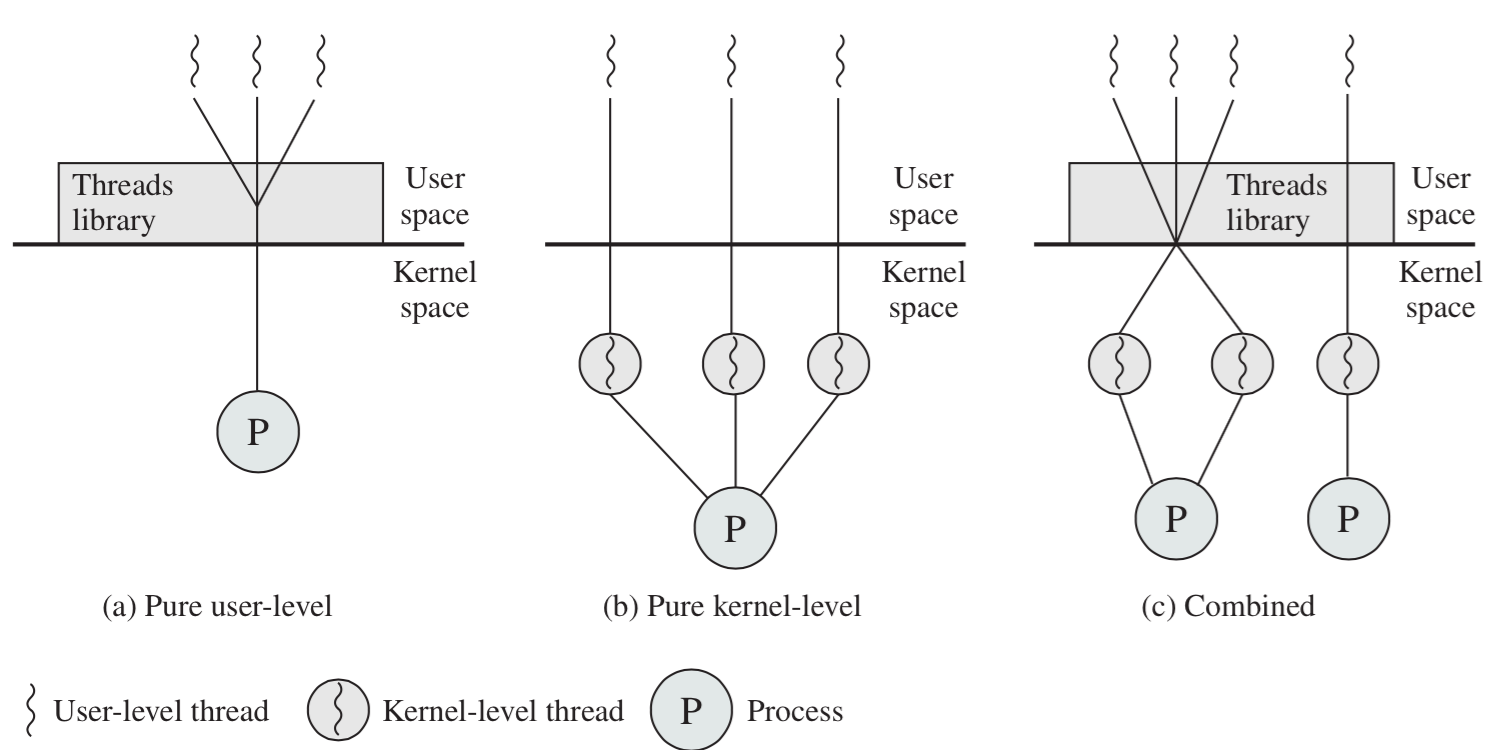
\includegraphics[width=0.85\textwidth]{images/thread-types.png}
\end{center}

\end{frame}

\begin{frame}
\frametitle{Thread Libraries}

If the operating system in question does not support threads, we can still have multithreaded programming. 

User level threads in some sort of threads library. 

The library handles creation, management, and cleanup of threads. 

The kernel is unaware of the existence of the user level thread.

It is the responsibility of the library/application to manage threads. 


\end{frame}

\begin{frame}
\frametitle{User Level Threads}

There are three advantages to using user-level threads~\cite{osi}:
\begin{enumerate}
	\item Thread switches do not require kernel mode privileges.
	\item Scheduling can be something the program decides.
	\item Portability.
\end{enumerate}


\end{frame}

\begin{frame}
\frametitle{User Level Threads}
The kernel thinks there is only one thread for that process.

If any thread blocks, the whole process is blocked.

Solution: \alert{jacketing}.\\
\quad Conversion of a blocking system call into a non-blocking one.

The jacketing routine checks if it's a blocking request.\\
\quad If so, decides to switch to another thread.

\end{frame}

\begin{frame}
\frametitle{Windows Threads}

The kernel level threads approach is taken by Windows. 

The kernel is responsible for all thread management.

If one thread in a process is blocked, the others may continue. 

Windows kernel routines themselves may be multithreaded.

\end{frame}

\begin{frame}
\frametitle{Relationship Model}

To look at this from another angle, we can consider the relationships.

There are three: Many-To-One, One-To-One, and Many-To-Many.

\begin{center}
	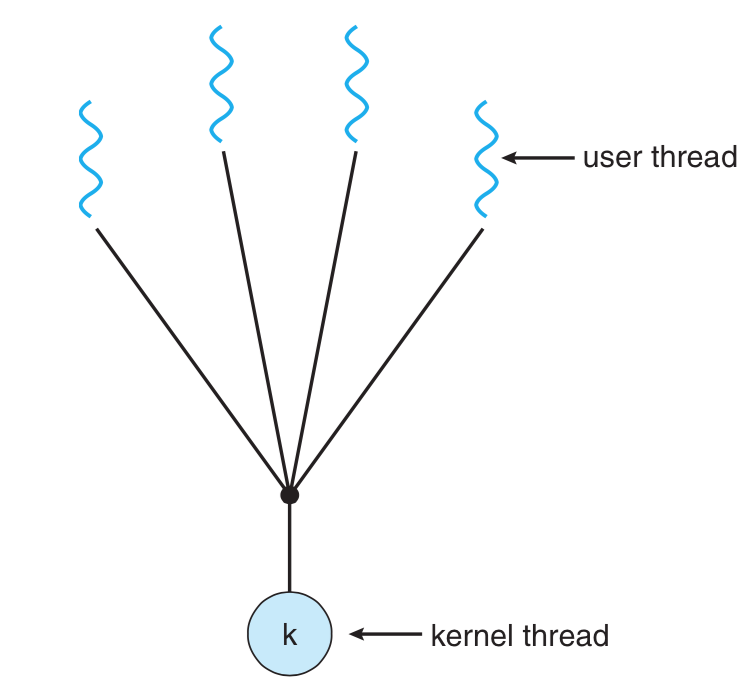
\includegraphics[width=0.32\textwidth]{images/threads-manytoone.png}
	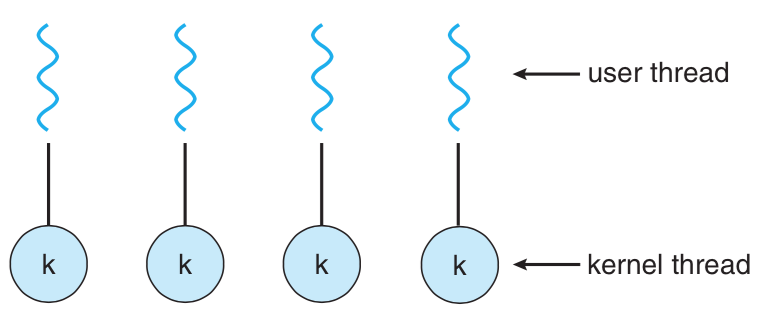
\includegraphics[width=0.32\textwidth]{images/threads-onetoone.png}
	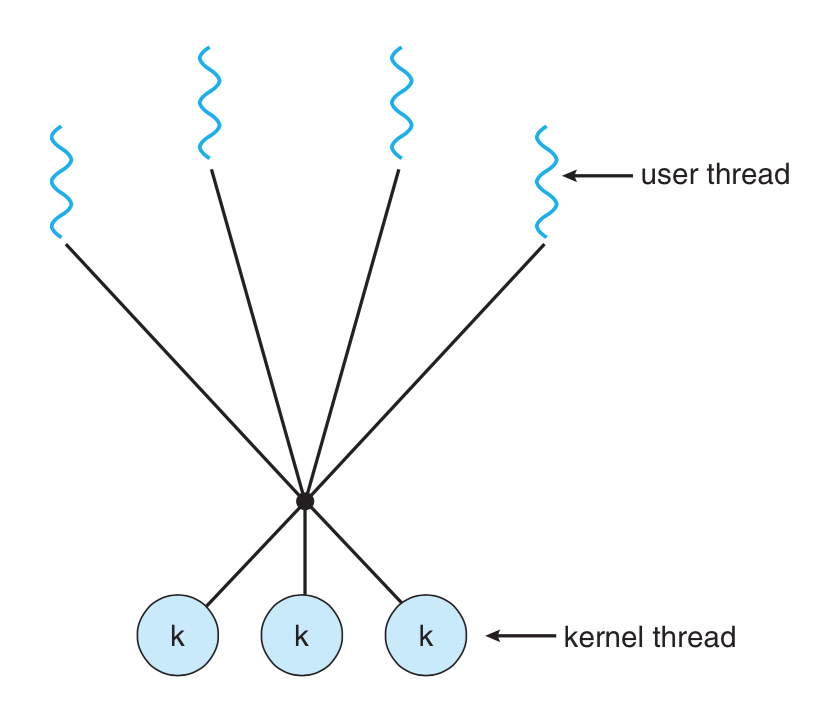
\includegraphics[width=0.32\textwidth]{images/threads-manytomany.png}
\end{center}

\end{frame}

\end{document}

